\documentclass{article}
\usepackage[portuguese]{babel}
\usepackage[utf8]{inputenc}
\usepackage[T1]{fontenc}
\usepackage{oz} %Z notatio
\usepackage{listings}
\usepackage{verbatim}
\usepackage{hyperref}
\usepackage{graphicx}
\usepackage{titling}

\hypersetup{
    colorlinks=true,       % false: boxed links; true: colored links
    linkcolor=red,          % color of internal links (change box color with linkbordercolor)
    citecolor=green,        % color of links to bibliography
    filecolor=magenta,      % color of file links
    urlcolor=black           % color of external links
}

\pretitle{%
  \begin{center}
  \LARGE
  
\includegraphics[scale=0.4]{um_logo}\\[\bigskipamount]
}
\posttitle{\end{center}}

\title{MathemaGrids Solver\\ implementation using Z3 SMT Solver}
\author{José Pereira \texttt{pg27748} 
		\\ Marta Azevedo \texttt{pg27763}
		              \\ Tiago Brito \texttt{pg27724}}
\begin{document}
\begin{titlepage}
\maketitle
\end{titlepage}

\section{MathemaGrids}

\paragraph{} 
O {\sc{MathemaGrids}} é um puzzle onde o objectivo é preencher uma tabela $mxm$ com inteiros entre 1 e m*m, de tal maneira que cada um desses números aparece apenas uma vez. 
\\

Para além disso, a posição dos números deve respeitar as operações que já estão presentes no tabuleiro.
\\
Neste relatório, pretendemos descrever de forma clara a nossa implementação.
\\

Para isso vamos usar como exemplo o seguinte tabuleiro:
\begin{center}
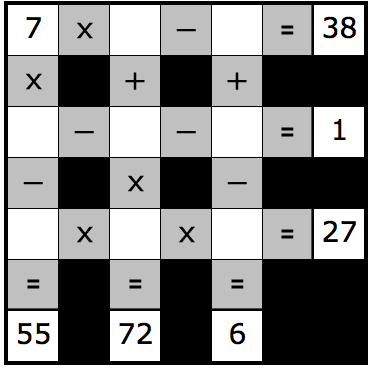
\includegraphics[scale=0.4]{exemplo_mathemagrids}
\end{center}

Neste exemplo, já é dada uma {\it{hint}}, o $7$ que aparece na primeira linha, primeira coluna.

\section{Implementação}
\subsection{SMT Solver}
Como {\sc{SMT-solver}} estamos a usar o {\sc{z3}} Theorem Prover da Microsoft Research. Este, é usado em vários softwares de verificação formal. 

\subsection{Linguagem de Programação}
Como linguagem de interface com o {\sc{z3}} preferimos usar o {\sc{python}} {\sc{z3Py}} devido à sua {\sc{API}} fácil de usar e devido a ser uma linguagem simples e eficaz para o que queriamos fazer.

\subsection{Interface Gráfica}
No que toca à Interface Gráfica, foi feito um trabalho de pesquisa prévio pelas mais diversas frameworks para python e, no final, decidimos usar o {\sc{Kivy}} v1.9.0. 
\\

{\sc{Kivy}} tráta-se de uma Framework multi-plataforma para Python, correndo em Linux, Windows, OS X, Android e iOS. É uma ferramenta grátis e é ``GPU Accelerated". 

\section{Estrutura}
O Projeto é dividido em cinco módulos:
\begin{itemize}
\item{\texttt{game.py}

Este é o módulo principal do projecto, sendo responsável pela inuficação de todas as funcionalidades e funcionamento das mesmas.}

\item{\texttt{gameGUI.py}

Este é o módulo responsável por toda a interface grática. É ele quem inicializa o jogo e utiliza os restantes módulos de forma a executar as respetivas funções.}

\item{\texttt{generate\_board.py}

Trata-se do módulo responsável por criar tabuleiros e gerar as suas soluções utilizando o $Z3$.}

\item{\texttt{parsing.py}

É o módulo responsável por fazer a leitura de um ficheiro de texto. Neste módulo está implementada uma gramática (que utiliza a biblioteca {\it{pyparsing}}) de forma a validar o input do ficheiro.}

\item{\texttt{solveMathemaGrids.py}

Este trata-se de um módulo de suporte onde temos algunas funções auxiliares bem como a função que nos permite usar o {\it{Solver}} para obter a solução de um tabuleiro lido de ficheiro.}
\end{itemize}

\section{Execução}
Para a execução do programa basta executar na consola :
\begin{verbatim}
$ python game.py
\end{verbatim}

Existem flags opcionais que podem ser usadas:
\begin{itemize}
\item{ {\bf{- -console}} : permite a execução do software em modo consola. Deve ser seguido do nome/localização do ficheiro de input}
\end{itemize}

E tendo atenção ás ás seguintes dependencias:
\begin{itemize}
\item{ {\bf{Python}} : Disponivel já de raiz com o Linux e OSX, mas também disponivel para Windows.}
\item{ {\bf{Kivy}} : Necessário $Kivy$ v1.9.0 disponivel no website {\url{http://kivy.org/}}.
\\
Para instalar:
\begin{verbatim}
$ sudo add-apt-repository ppa:kivy-team/kivy
$ sudo apt-get install python-kivy
\end{verbatim}
}
\item{ {\bf{Z3}} : Disponivel em {\url{https://github.com/Z3Prover/z3}}:}
\item{ {\bf{pyparsing}} :  Disponivel em {\url{http://pyparsing.wikispaces.com/}} e com instalação simples através do pip, bastando fazer 
\begin{verbatim}
$ pip install pyparsing
\end{verbatim}
}
\end{itemize}

\section{Ficheiros input}

\paragraph{} 

Para representar um tabuleiro de {\sc{MathemaGrids}} (o do exemplo) usamos o seguinte ficheiro de texto:
\begin{center}
\begin{verbatim}
7*.-.=38
*,+,+
.-.-.=1
-,*,-
.*.*.=27
=,=,=,=
55,72,6
\end{verbatim}
\end{center}

Os $"."$ representam os espaços que têm que ser preenchidos com números e as $","$ representam os espaços que, apesar de existirem no tabuleiro, não podem ser inseridos com números. 
\\

Também estão representadas as operações sendo o {\bf{*}} a multiplicação, o  {\bf{+}} a soma, {\bf{-}} a subtração e {\bf{/}} a divisão. 

%\subsection{Ficheiros output}
%\paragraph{} 
%O {\sc{MathemaGrids}} dá como output um ficheiro com a representação da matriz obtida e os %valores que as linhas e as colunas que respeitam as operações dadas como imput.


%O do exemplo :
%\begin{center}
%\begin{verbatim}
%{\bf{------> falta o output}}
%\end{verbatim}
%\end{center}

\subsection{Codificação do {\sc{MathemaGrids}}}
\paragraph{} Para codificar o puzzle,usamos as seguintes propriedades \\
(descritas em {\url{https://www.brainbashers.com/mathemagrids.asp}}):
 \begin{enumerate}
 \item Usar todos os digitos de 1 a $m*m$ (no nosso exemplo, até $9$);
 \item Nenhum número pode ser repetido;
 \item As operações são feitas da esquerda para a direita e de cima para baixo, sendo a ordem de prioridade normal da matemática ignorada;
 \item Não podem existir divisões por 1 nem multiplicações por 1;
\item Em nenhum ponto, os resultados intermédios do cálculo são valores infeiores a zero.
 \end{enumerate}

As variaveis $x$\_$membros$ e $y$\_$membros$ representam a quantidade de espaços em que o jogador pode inserir números nas linhas e nas colunas respetivamente. As regras usadas são:

 \begin{enumerate}
 \item 
\begin{verbatim}
max_size = [And(1 <= x[j][i], x[j][i] <= size * size) 
for i in range(size) for j in range(size)]
\end{verbatim}

 \item \small{(No ficheiro generate$\_$board.py)}

\begin{verbatim}
unique = [Distinct([x[j][i] for i in range(size) for j in range(size)])]
\end{verbatim}

 \item Para garantir que as operações são feitas na ordem correta, escrevemos as equações horizontais e verticais que, neste exemplo são : \\
\begin{itemize}
\item {\bf{Equações Verticais:}}
\begin{verbatim}
(7 * x_1_2) - x_1_3 = 55
(x_2_1 + x_2_2) * x_2_3 = 72
(x_3_1 * x_3_2) - x_3_3 = 6
\end{verbatim}
\item {\bf{Equações Horizontais:}}
\begin{verbatim}
(7 * x_2_1) - x_3_1 = 38
(x_1_2 - x_2_2) - x_3_2 =1
(x_1_3 * x_2_3) * x_3_3 = 27
\end{verbatim}
\end{itemize}

\item 
\small{
\begin{verbatim}
    not_one_exceptions = []
    for i in range(len(board)):
        for j in range(len(board[i])):
            if str(board[i][j]) == "/" or str(board[i][j]) == "*":
                if i % 2 == 0:
                    not_one_exceptions.append(Not(x[i/2][(j+1)/2] == 1))
                else:
                    not_one_exceptions.append(Not(x[(i+1)/2][j/2] == 1))
\end{verbatim}
}

\item Como a operação crítica para isto acontecer é apenas a subtração: 

\begin{verbatim}
bigger_than_zero = []
for i in range(len(board)):
 for j in range(len(board[i])):
     if i % 2 == 0:
         if board[i][j] == '-':
             if j == 1:
                 bigger_than_zero.append(Not(x[i/2][(j-1)/2] - x[i/2][(j+1)/2] < 0))
             else:
                 equation = ""
                 for n in range(j):
                     if n > 2 and str(board[i][n]) != "." and not(board[i][n].isdigit()):
                         equation = "("+equation+")"+str(board[i][n])
                     else:
                         if board[i][n] == "." or board[i][n].isdigit():
                             equation += "x["+str(i/2)+"]["+str(n/2)+"]"
                         else:
                             equation += board[i][n]
                 equation = equation + "-" + "x[" + str(i/2) + "][" + str((j+1)/2)+"]" + ">0"
                 bigger_than_zero.append(eval(equation))
\end{verbatim}

\item Esta regra serve para garantir que o y em $x/y$ é um multiplo do $x$. Caso contrário, por exemplo $6/2=3=7/2$
\begin{verbatim}
 multiple = []
    for i in range(len(board)):
        for j in range(len(board[i])):
            if i % 2 == 0:
                if board[i][j] == '/':
                    multiple.append(x[i/2][(j-1)/2] % x[i/2][(j+1)/2] == 0)
            else:
                if board[i][j] == '/':
                    multiple.append(x[(i-1)/2][j/2] % x[(i+1)/2][j/2] == 0)
\end{verbatim}

 \end{enumerate}

No final, é enviado para o solver:
\begin{verbatim}
 rules = unique+bigger_than_zero+not_one_exceptions+max_size+multiple
\end{verbatim}

\section{{\it{generate$\_$board.py}}}
\subsection{Hints}

As hints foram adicionadas ao nosso projeto com o objetivo de ajudar o jogador a chegar mais rapidamente à solução. Como tal, na opção ``{\it{Settings}}'' podemos selecionar duas opções relativamente a este assunto:
\begin{enumerate}
\item Ativar hints
\item Hints preenchem apenas campos vazios
\end{enumerate}

Se a {\bf{opção 1}} estiver ativada, quando clicarmos em ``{\it{Hint}}'' no menu inicial é sugerido um número para um espaço (mesmo que este já tenha sido preenchido pelo utilizador).
\\

Se ativarmos a {\bf{opção 2}}, as sugestões são apenas dados em campos que não tenham sido preenchidos, mesmo que as opções que o utilizador inseriu estejam erradas. 


\subsection{Geração de tabuleiros}

A geração de tabuleiros é feita recebendo como argumento o tamanho do tabuleiro e é criada uma matriz com esse tamanho. Por exemplo, para gerar um tabuleiro do mesmo tamanho que o exemplo, o número seria 3.
\\

As operações estão guardadas num array e, de forma aleatoria, são colocadas na matriz. 
\\

A seguir, e em conjunto com as regras da secção {\bf{3.3}} é enviada a matriz ao {\it{solver}}. Caso o problema seja satisfazivel, é considerada essa matriz uma matriz válida. É enviada para uma função que calcula os valores que vão estar na última linha e última coluna (depois do $=$). 
\\

Depois do tabuleiro pronto, é enviado para um ficheiro de texto onde é armazenada com especificado na secção {\bf{3.1}}.
\end{document}